\documentclass[draft=false, titlepage]{article}

\usepackage[utf8]{inputenc}
\usepackage{graphicx} % graphicx is for including images
\usepackage{amsmath} % equation arrays, boxed equations, more symbols
\usepackage{mathabx} % double/triple integrals
% hyperref will turn the table of contents, etc. into hyperlinks. You can use them to jump to sections in the pdf
\usepackage{hyperref}
\hypersetup{
    colorlinks=true,
    pdfborder={0 0 0},
}
% geometry is used to set the page margin, otherwise the margin is (in emi's opinion) too big
\usepackage[margin=1in]{geometry}

% let's define some custom commands
\newcommand{\gradient}{\vec{\nabla}}
\newcommand{\deldelt}{\frac{\partial}{\partial t}}
\newcommand{\partialfrac}[2]{\frac{\partial #1}{\partial #2}}
% There is a package collision where I cannot import a closed triple integral symbol. It causes the \nabla used as a gradient operator to appear incorrectly as a big black blob.
\newcommand{\volumeint}{\iiint_V}

\title{Liebeck's 158 Notes, 21st Century Edition}
\author{Transcribed from Professor Liebeck's notes PDF\\
	\small Emiko Soroka}
\date{Last Compiled: \today\linebreak\linebreak
	\small Revision: 0.1\\
	Release Notes: Working on it...}

\begin{document}
\maketitle
\tableofcontents
\listoffigures
\listoftables
\pagebreak

% PRAGMA MARK NEW SECTION, page 1 % Page number corresponds to Liebeck's original
\section{Aerodynamics Review}
\subsection{Velocity and Streamlines}
"Velocity at a point B within a gluid is the velocity of an infinitesimally small fluid element as it sweeps through B.
The path of a fluid element is called the streamline.

\begin{figure}[ht]
	\centering
	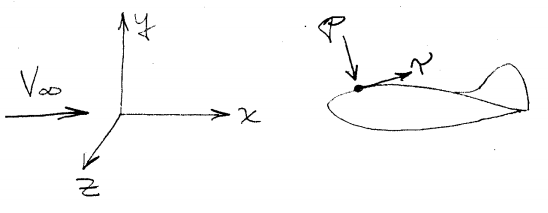
\includegraphics[width=0.5\linewidth]{Figures/p2_flowfield.PNG}
	\caption{$P$ and $\tau$ on a body in a flow field}
	\label{fig:p2_flowfield}
\end{figure}
\begin{gather*}
P = P(x,y,z)\\
\rho = \rho(x,y,z)\\
T = T(x,y,z)\\
\vec{V} = \vec{V}(x,y,z)
\end{gather*}
Knowledge of $P,\ \rho,\ T,\ \vec{V}$ as functions of x,y,z completely defines the flow field.

\subsubsection{Aerodynamic Forces}
Knowledge of $p$ and $\tau$ on the surface of a body completely defines all aerodynamic forces on the body.

\subsection{Basic Aerodynamics}
\begin{figure}[ht]
	\centering
	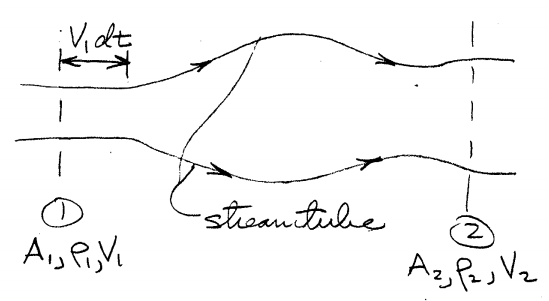
\includegraphics[width=0.5\linewidth]{Figures/p3_streamtube.PNG}
	\caption{Fluid flow in a streamtube}
	\label{fig:p3_streamtube}
\end{figure}
Continuity: conservation of mass.\\
Weight: $w = density\ \cdot volume$\\
In Figure \ref{fig:p3_streamtube}: $dw_w = \rho (V_1 dt \cdot A_1)$
\begin{gather*}
\text{Mass flow rate} = \frac{dw_1}{dt} = \dot{m_1} = \rho_1 A_1 V_1 (\frac{kg}{sec},\ \frac{slug}{sec})\\
\text{Similarly} \quad \frac{dw_2}{dt} = \rho_2 A_2 V_2
\end{gather*}
Since there can be no flow across the streamtube (by definition)
\begin{equation*}
\frac{dw_1}{dt} = \frac{dw_2}{dt} \rightarrow \boxed{\rho_1A_1V_1 = \rho_2A_2V_2}
\end{equation*}
This is the continuity equation for steady flow.

\subsection{Compressibility}
\paragraph*{} All fluids are "compressible", including water. Compressibility means that the fluid density can vary with both time and position. There are cases where a fluid can be assumed to be incompressible with good results. Flow of liquids is a common example. Also, the flow of gases such as air can also be taken as incompressible as long as the velocity remains below $\approx 225\ mph$ or $100\ m/s$.
\paragraph*{} The assumption of incompressible flow simplifies the continuity equation:
\begin{gather*}
\rho = const \rightarrow \rho_1 = \rho_2\\
V_1A_1 = V_2A_2 \quad \text{or} \quad V_2 = \big(\frac{A_1}{A_2}\big)V_1
\end{gather*}

\subsection{Momentum Equation}
\begin{figure}[ht]
	\centering
	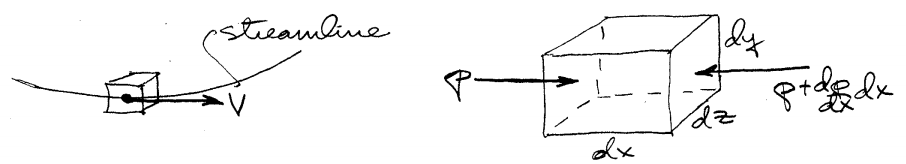
\includegraphics[width=0.8\linewidth]{Figures/p5_momentum.PNG}
	\caption{Momentum on a fluid element along a streamline}
	\label{fig:p5_momentum}
\end{figure}
Newton's Law: Force = mass * acceleration
\paragraph*{} Consider fluid element $dx\ dy\ dz$ moving along a streamline with velocity $V$. Forces on this element include:
\begin{enumerate}
	\item pressure normal to all six faces
	\item friction tangential to all six faces
	\item gravity acting on the mass
\end{enumerate}
To begin, assume that friction and gravitational forces are negligible.
\begin{align*}
\text{Pressure force on left face} &\quad = pA = p dy\ dz\\
\text{Since pressure may vary with position}&\\
\text{Pressure force on right face} &\quad = (p + \frac{dp}{dx}dx) dy\ dz\\
\text{The force F in the x-direction is}
&\quad F=p dy\ dz - (p + \frac{dp}{dx}dx)dy\ dz\\
&\quad F = -\frac{dp}{dx}(dx\ dy\ dz)\\
\text{Mass of fluid in element} &\quad = \rho (dx\ dy\ dz)\\
\text{Acceleration of element} &\quad a = \frac{dV}{dt},\quad \text{Also } V = \frac{dx}{dt}\\
\rightarrow &\quad a = \frac{dV}{dt} = \frac{dV}{dx}\frac{dx}{dt} = \frac{dV}{dx}V\\
\text{Applying Newton's 2nd law:} F=ma &\quad -\frac{dp}{dx}(dx\ dy\ dz) = \rho(dx\ dy\ dz) V \frac{dV}{dx}\\
\rightarrow &\quad dp = \rho V dV = 0
\end{align*}
This is the momentum equation for frictionless (inviscid) flow.
\begin{figure}[ht]
	\centering
	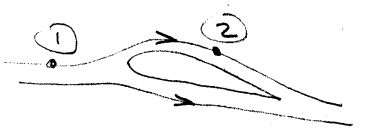
\includegraphics[width=0.3\linewidth]{Figures/p6_flowOnAirfoil.PNG}
	\caption{Flow at points 1 and 2 on an airfoil}
	\label{fig:p6_flowOnAirfoil}
\end{figure}
\paragraph*{} Consider the flow about an airfoil, and assume that it is incompressible. Integrate the momentum equation between 1 and 2 in Figure \ref{fig:p6_flowOnAirfoil}.
\begin{gather*}
\int_{p_1}^{p_2} dp + \rho \int_{V1}^{V_2} V dV = 0\\p_2 - p_1 + \rho\big(\frac{V_2^2}{1}-\frac{V_1^2}{2}\big) = 0\\
p_2 + \rho\frac{V_2^2}{2} = p_1 + \rho \frac{V_1^2}{2}\\
\text{or } \boxed{p + \rho \frac{V^2}{2} = \text{const. along a streamline}}
\label{eq:Bernoulli}
\end{gather*}
which is called Bernoulli's equation. This applies only for incompressible, inviscid flows.
\paragraph*{Note:} The continuity and momentum equations relate conditions along a streamline, typically between two distinct points. The equation of state defines a relation between $\rho,\ p,\ \& T$ at a specific point.

\subsection{Note on Units}
\begin{align*}
\text{Dynamic Pressure} &\quad = \frac{1}{2}\rho V^2\\
\rightarrow &\quad \frac{mass}{l^3} \cdot \frac{l^2}{d^t} = \frac{F}{l^2}\\
\text{Recall }&\quad F=ma\\
\text{1 pound} &\quad = 1\ slug \cdot 1\frac{ft}{sec^2} \text{ or } 1\ slug = \frac{1\ pound}{1\ ft/sec^2}\\
\frac{1}{2}\rho V^2 &\quad = \frac{slugs}{ft^2} \cdot \frac{ft^2}{sec^2} = \frac{pound}{ft/sec^2}\cdot \frac{1}{ft^3}\cdot \frac{ft^2}{sec^2} = \frac{pound}{ft^2}\\
1\ newton = 1\ kg \cdot 1\ meter/sec^2 &\quad 1\ kg = \frac{1N}{1m/sec^2}\\
\frac{1}{2}\rho V^2 &\quad = \frac{kg}{m^3}\cdot \frac{m^2}{sec^2} = \frac{M}{m/sec^2}\cdot \frac{1}{m^3}\cdot \frac{m^2}{sec^2} = \frac{N}{m^2}
\end{align*}

\section{Applications}
\subsection{Low-Speed Wind Tunnels}
\begin{figure}[ht]
	\centering
	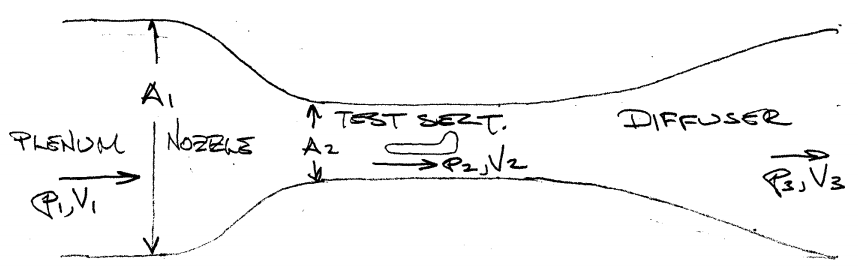
\includegraphics[width=0.7\linewidth]{Figures/p9_lowSpeedWindTunnel.PNG}
	\caption{Flow in a low-speed wind tunnel}
	\label{fig:p9_lowSpeedWindTunnel}
\end{figure}

\begin{gather*}
\text{Assume incompressible flow. Then: } \rho = const\\
\text{From continuity: } A_1V_1 = A_2V_2 \rightarrow V_2 = \big(\frac{A_1}{A_2}\big)V_1\\
\text{From Bernoulli's Equation: } p_1 + \frac{1}{2}\rho V_1^2 = p_2 + \frac{1}{2}\rho %V_2^2\\
V_1 < V_2 \rightarrow p_1 > p_2\\
\text{Solving for } V_2^2\\
V_2^2 = \frac{2}{\rho}(p_1-p_2) + V_1^2 = \frac{2}{\rho} (p_1-p_2) + \big(\frac{A_2}{A_1}\big)^2 V_2^2\\
\boxed{V_2 = \sqrt{\frac{2(p_1-p_2}{\rho\big[ 1-(A_2/A_1)^2 \big]}}}
\end{gather*}

\subsection{Measurement of Pressure with a Manometer}
\begin{figure}[ht]
	\centering
	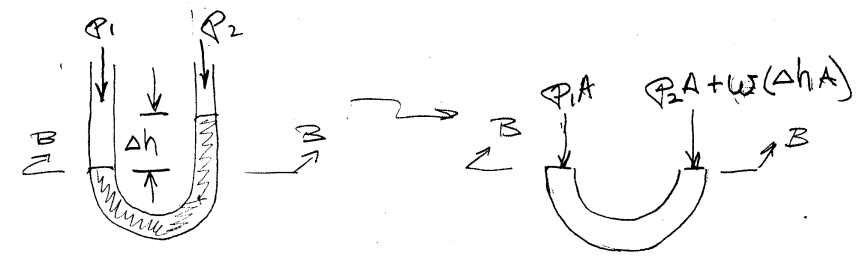
\includegraphics[width=0.7\linewidth]{Figures/p10_manometers.PNG}
	\caption{Pressure measurement using a manometer}
	\label{fig:p10_manometers}
\end{figure}
\begin{gather*}
\rho_F = \text{density of manometer fluid}\\
\text{For equilibrium} \quad p_1A = p_2A + w\Delta h A\\
\boxed{p_1-p_2 = w\Delta h = \rho_F g \Delta h}
\end{gather*}
\paragraph*{Note:} Pressures are commonly (and often most accurately) measured as "pressure differences".

% PRAGMA MARK page 11
\subsection{Measurement of Airspeed}
We desire to obtain the flow velocity by measurements at a single point. Then, we must first define "total pressure" as the pressure that would exist if the flow were slowed isentropically to zero velocity.
\paragraph*{Pitot Tube}
The pitot tube measures $p_0$, the total pressure. (Note there can be no flow out of the tube, therefore $V=0$.)
\paragraph*{Pitot-Static Tube}
Here, the gage measures the pressure difference $p_0-p$.

\begin{figure}[ht]
	\centering
	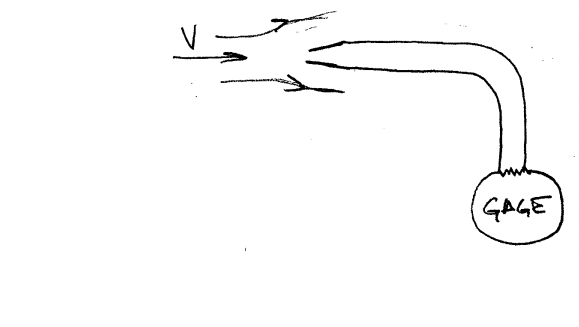
\includegraphics[width=0.4\linewidth]{Figures/p11_pitot.PNG}
	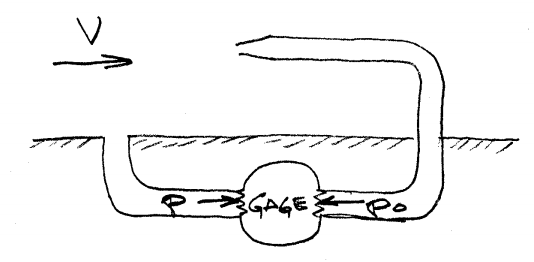
\includegraphics[width=0.4\linewidth]{Figures/p11_pitotStatic.PNG}
	\caption{Pitot and pitot-static tubes}
	\label{fig:p11_pitotStatic}
\end{figure}

For incompressible flow, Bernoulli's Equation gives
\begin{equation*}
p + \frac{1}{2}\rho V^2 = p_0 rightarrow \text{Static} + \text{Dynamic} = \text{Total}
\end{equation*}
From which we define "dynamic pressure" as
\begin{equation}
q = \frac{1}{2}\rho V^2
\label{eq:dynamicPressure}
\end{equation}
Bernoulli's equation can be solved for V
\begin{equation}
\boxed{V = \sqrt{2\frac{p_0-p}{\rho}}}
\label{eq:vFromBernoulli}
\end{equation}
\begin{figure}[ht]
	\centering
	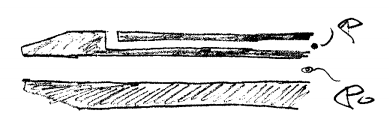
\includegraphics[width=0.4\linewidth]{Figures/p12_pitotStatic.PNG}
	\caption{Pitot-static tube}
	\label{fig:p12_pitotStatic}
\end{figure}
A pitot-static tube (Figure \ref{fig:p12_pitotStatic}) can be used to obtain the velocity at a point in the flow.
\paragraph*{Note:} You must be very careful to align the probe with the velocity vector, or the static pressure reading will be in error.
\paragraph*{} Pitot and pitot static tubes can be used to measure velocity in wind tunnels The difficulty is in accurage measurement of static pressure (flow in test section, open test section, etc.) % There is some illegible word in this sentence

\subsubsection{Airplane Airspeed}
\begin{gather*}
\text{The pitot-static probe gives} \quad V_e = \sqrt{2\frac{p_0-p}{\rho_s}}\\
V_e = \text{equivalent airspeed}\\
\rho_s = \text{sea level density}\\
V_{TRUE} = V_e \big( \frac{\rho_s}{\rho_{ACTUAL}} \big)^{1/2}
\end{gather*}

% PRAGMA MARK PAGE 14
\subsection{Viscous Flow}
\begin{figure}[ht]
	\centering
	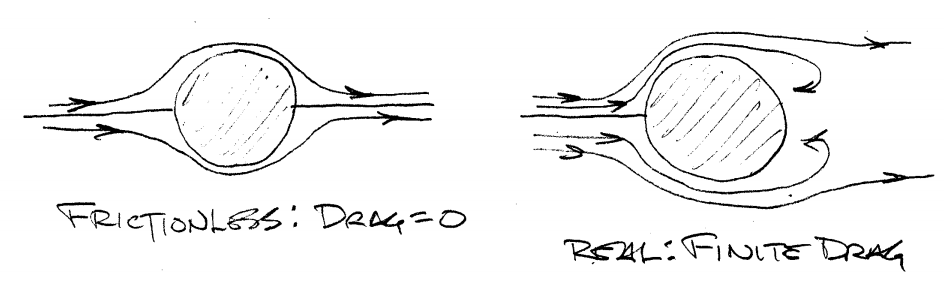
\includegraphics[width=0.8\linewidth]{Figures/p14_frictionDrag.PNG}
	\caption{Flow on a circular cylinder with real friction drag}
	\label{fig:p14_frictionDrag}
\end{figure}
Consider flow about a circular cylinder (Figure \ref{fig:p14_frictionDrag}). Frictionless flow will show zero drag about any body. This is called "d'Alembert's paradox".
\paragraph*{}In the case of a real flow, viscous effects produce drag from two primary sounrces:
\begin{enumerate}
	\item \textbf{Skin Friction Drag}  - a main source of drag on streamlined bodies such as wings
	\item \textbf{Separation Drag} - drag of bluff bodies such as a cylinder or a stalled wing.
\end{enumerate}

\subsection{Boundary Layer}
Thus far, analyses using Bernoulli's equation have assumed flow to have a finite, non-zero velocity at the surface of a body. In fact, there exists a very thin layer next to the body where velocity varies from a finite value to zero at the body surface. This is called the "boundary layer" (Figure \ref{fig:p15_boundaryLayer}).
\begin{figure}[ht]
	\centering
	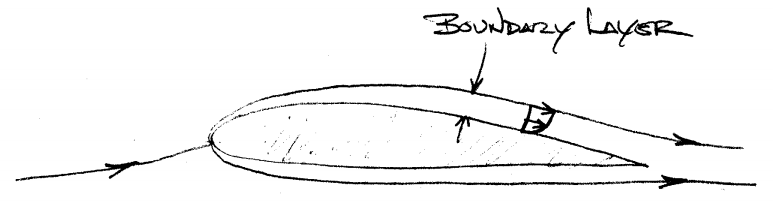
\includegraphics[width=0.5\linewidth]{Figures/p15_boundaryLayer.PNG}
	\caption{Boundary layer on an airfoil}
	\label{fig:p15_boundaryLayer}
\end{figure}
\paragraph*{} The boundary layer is a viscous phenomenon where friction between the flow and the body auses its development. Typically, for streamlined bodies, all viscous effects may be regarded as confined to this very thin layer ,and the flow field outside can be calculated using the frictionless relationships such as Bernoulli's Equation.
\paragraph*{} Also, the static pressure across the boundary layer is constant. This provides of fundamental theoretical concept as introduced in 1906. Analysis of a flow field can be broken-up into two portions: %there are more illegible things here
\begin{enumerate}
	\item The boundary layer where viscous considerations predominate.
	\item The outer region flow where frictionless analysis (potential) flow can be assumed.
\end{enumerate}

\subsubsection{Details of a Boundary Layer}
\begin{figure}[ht]
	\centering
	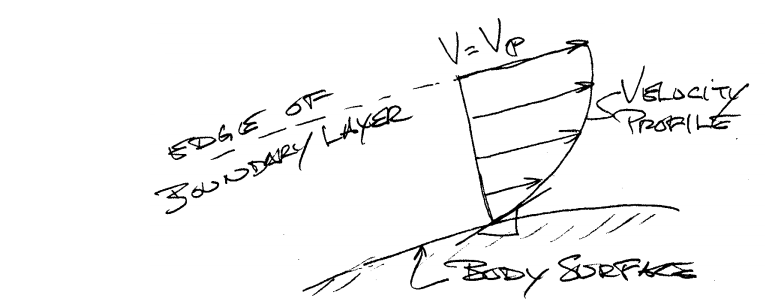
\includegraphics[width=0.6\linewidth]{Figures/p17_velocityProfile1.PNG}
	\caption{Boundary layer profile on a body surface}
	\label{fig:p17_boundaryLayer1}
\end{figure}
\begin{gather*}
\tau_w = \mu \big( \frac{dV}{dy} \big)_{y=0}\\
\tau_w = \text{shear stress at surface (force/unit area)}\\
\mu = \text{coefficient of viscosity}\\
\frac{dV}{dy}\big)_{y=0} = \text{slope of velocity gradient of surface.}
\end{gather*}
\subsubsection{Laminar vs. Turbulent Boundary Layers}
\begin{gather*}
\tau = \mu \big(\frac{dV}{dy}\big)_{y=0}\\
\frac{dV}{dy}\big)_{y=0,\ lam.} < \frac{dV}{dy})_{y=0,\ turb.}\\
\text{Then}\quad \tau\big)_{LAM} < \tau\big)_{TURB}
\end{gather*}
\begin{figure}[ht]
	\centering
	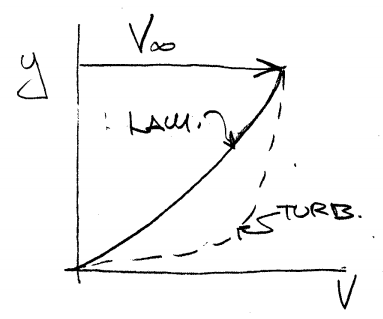
\includegraphics[width=0.3\linewidth]{Figures/p17_velocityProfile2.PNG}
	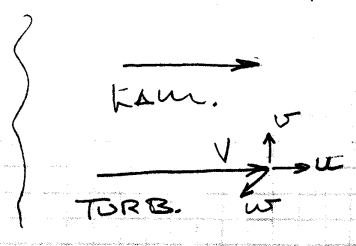
\includegraphics[width=0.3\linewidth]{Figures/p17_velocityProfile3.PNG}
	\caption{Boundary layer profile for laminar and turbulent flow}
	\label{fig:p17_boundaryLayer23}
\end{figure}

% PRAGMA MARK PAGE 18
\subsection{Reynolds Number} (similarity parameter)
\begin{gather}
RN = \frac{\rho_\infty V_\infty x}{\mu_\infty} \rightarrow \frac{\text{Inertial Forces}}{\text{Viscous Forces}}\\
x = \text{characteristic length}\\
\mu = 1.7984\cdot 10^{-5} kg/m\cdot sec = 3.7373 \cdot 10^{-7} slug/ft\cdot sec
\label{eq:Reynolds}
\end{gather}
\subsubsection{Transition}
The change in the state of a boundary layer from laminar to turbulent. Reference is often made to a "transition point", however transition actually occurs over a region of finite length which becomes significant for $RN < 10^6$.
\paragraph*{} Factors affecting transition include:
\begin{enumerate}
	\item $RN \rightarrow $ Increasing $RN$ moves transition forward.
	\item Surface roughness $\rightarrow$ increasing moves transition forward.
	\item Pressure gradient $\rightarrow dp/dx > 0 \rightarrow $ forward, $dp/dx < 0 \rightarrow$ aft.
\end{enumerate}

\subsection{Skin Friction Coefficient}
\begin{equation}
C_f = \frac{\tau_w}{\frac{1}{2}\rho_\infty V_\infty} = \frac{\tau_w}{q_\infty} = \frac{0.664}{\sqrt{RN_x}}\Big)_{LAM}
\label{eq:skinFriction}
\end{equation}
Note: $\tau =$ shear force / unit area = shear stress.\\
$q_\infty$ = normal force / unit area = pressure (dynamic).
\subsubsection{Skin Friction Drag Coefficient}
For a flat plate of length L:
\begin{equation}
D_f  = \int_0^L \tau_w dx,\quad \tau_w\Big)_{LAM} = \frac{0.664}{\sqrt{RN_x}}q_\infty
\label{eq:skinFrictionDrag}
\end{equation}

\begin{gather*}
\text{Define} C_{Df} = \frac{D_f}{q_\infty L}\\C_{Df}\Big)_{LAM} = 1.328/\sqrt{RN_L},\quad \delta\Big)_{LAM} = \frac{5.2x}{\sqrt{RN_x}}\\
C_{Df}\Big)_{TURB} = 0.074/(RN)^{0.2},\quad \delta\Big)_{TURB} = \frac{0.37x}{(RN_x)^{0.2}}\\
C_{Df}\Big)_{TURB} = 0.455/(\log_{10}RN_L)^{2.58}\\
\text{where } RN_L = \frac{\rho_\infty V_\infty L}{\mu_\infty}
\end{gather*}

\subsubsection{Laminar Boundary Layer}
\begin{align*}
\delta = frac{5.2l}{(RN_L)^{1/2}},\quad C_{fl} =& \frac{0.664}{(RN_l)^{1/2}},\quad C_f = \frac{\tau}{q_\infty}\\
D_f = \int_0^L \tau_w dx ,\quad \tau_=& \frac{0.664}{(RN_x)^{1/2}}q_\infty\\
C_{Df} = \frac{D_f}{q_\infty L}=& \frac{1}{q_\infty L}\int_0^L \tau_w dx\\
& \frac{1}{q_\infty L}\int_0^L \frac{0.664}{(RN_x)^{1/2}}q_\infty dx\\
& \frac{1}{L}\int_0^L \Big[ \frac{0.664}{(\rho_\infty V_\infty/\mu)^{1/2}}2L^{1/2} \Big]\\
C_{Df} =& \frac{1.328}{(RN_L)^{1/2}}
\end{align*}
Note: Shevell uses $C_f = C_{Df}$.

\end{document}